\documentclass{article}

\usepackage{graphicx}
\usepackage{tikz}
\usepackage{tikzsymbols}
\usetikzlibrary{calc,patterns,shapes.geometric}
\pagestyle{empty}
\usepackage[margin=0pt]{geometry}
\geometry{papersize={14in,12in}}

\def\centerarc[#1](#2)(#3:#4:#5){\draw[#1] ($(#2)+({#5*cos(#3)},{#5*sin(#3)})$) arc (#3:#4:#5);}

\begin{document}
	\begin{figure}
		\centering
		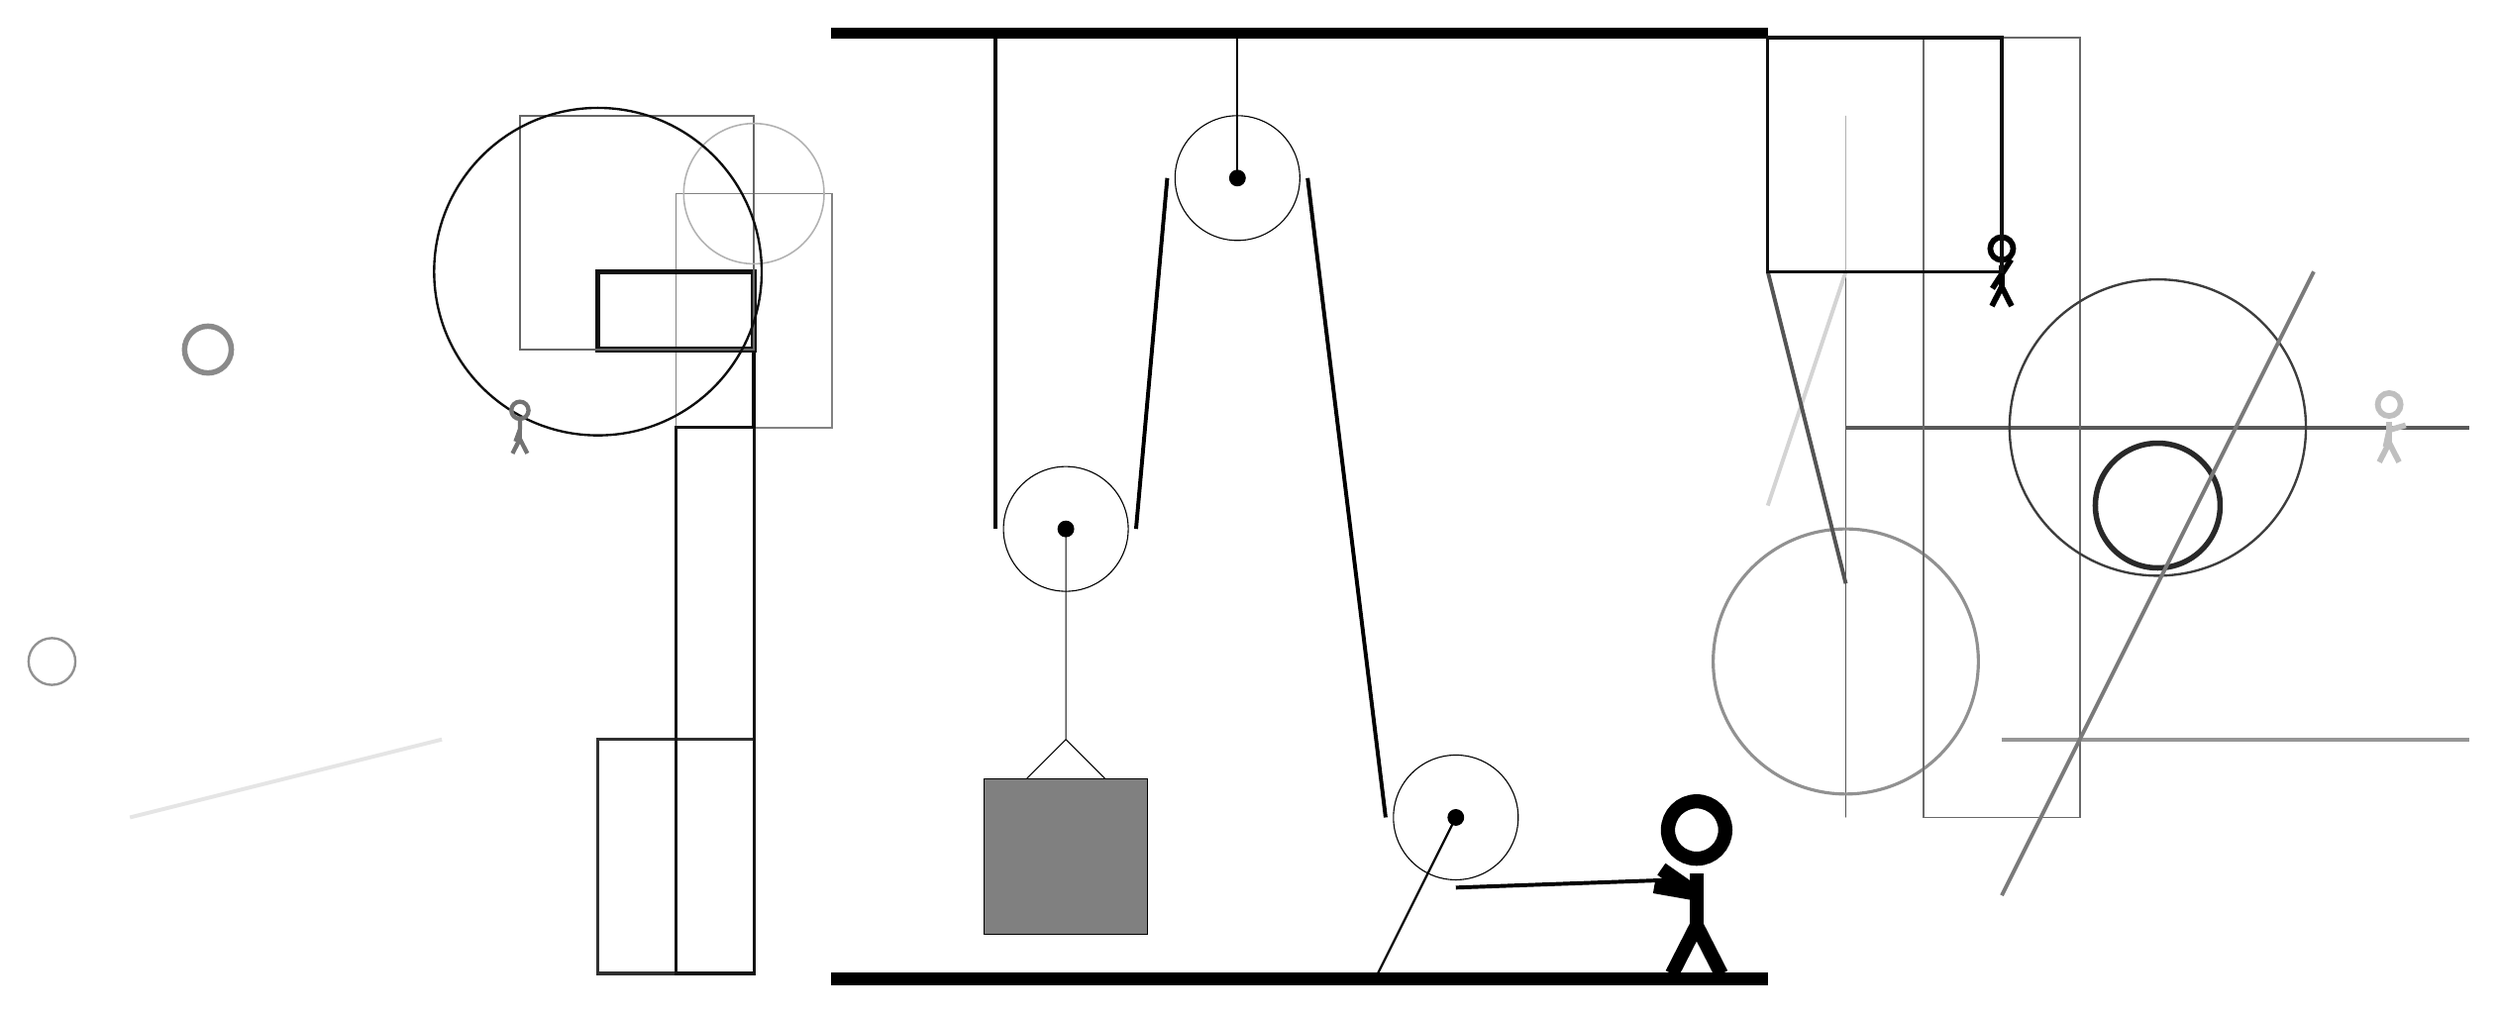
\begin{tikzpicture}
			%%%%% START %%%%%
			
			\draw[fill=black] (-2, 9) rectangle (10, 9.125);
			
			\draw (3.2, 7.2) circle (0.8);
			\draw[fill=black] (3.2, 7.2) circle (0.1);
			\draw[thick] (3.2, 7.2) -- (3.2, 9);
			
			\draw[line width=0.5mm, color=black!65](11, 4) -- (19, 4);
			
			\draw[line width=0.2mm, color=black!30] (11, -1) rectangle (11, 8);
			\draw[line width=0.4mm, color=black!81] (-3, 0) rectangle (-5, -3);
			\node[line width=0.6mm, color=black!25] at (18, 4) {\Strichmaxerl[4][78][16]};
			\draw[line width=0.2mm, color=black!49] (-2, 4) rectangle (-4, 7);
			\draw[line width=0.2mm, color=black!66] (11, -1) rectangle (11, 6);
			\draw[line width=0.5mm, color=black!17](10, 3) -- (11, 6);
			
			\draw [line width=0.4mm, color=black!43](11, 1) circle (1.7);
			\draw[line width=0.5mm, color=black!10](-7, 0) -- (-11, -1);
			\draw[line width=0.4mm, color=black!92] (-3, 4) rectangle (-4, -3);
			\draw[line width=0.5mm, color=black!67](10, 6) -- (11, 2);
			
			\draw [line width=0.3mm, color=black!43](-12, 1) circle (0.3);
			\draw[line width=0.6mm, color=black!98] (-3, 4) rectangle (-3, 5);
			
			\draw[line width=0.7mm, color=black!93] (-3, 6) rectangle (-5, 5);
			\draw[line width=0.2mm, color=black!59] (12, 9) rectangle (14, -1);
			\draw[line width=0.2mm, color=black!60] (-3, 5) rectangle (-6, 8);
			
			\node[line width=0.5mm, color=black!100] at (13, 6) {\Strichmaxerl[4][57][57]};
			\draw [line width=0.3mm, color=black!76](15, 4) circle (1.9);
			\draw[line width=0.5mm, color=black!41](13, 0) -- (19, 0);
			\draw [line width=0.2mm, color=black!30](-3, 7) circle (0.9);
			\draw [line width=0.3mm, color=black!95](-5, 6) circle (2.1);
			
			\draw [line width=0.7mm, color=black!84](15, 3) circle (0.8);
			
			\draw[line width=0.4mm, color=black!94] (10, 9) rectangle (13, 6);
			\node[line width=0.5mm, color=black!55] at (-6, 4) {\Strichmaxerl[3][70][89]};
			\draw[line width=0.5mm, color=black!52](13, -2) -- (17, 6);
			
			\draw [line width=0.7mm, color=black!46](-10, 5) circle (0.3);
			
			\draw (6, -1) circle (0.8);
			\draw[fill=black] (6, -1) circle (0.1);
			\draw[thick] (6, -1) -- (5, -3);
			
			\draw (1, 2.7) circle (0.8);
			\draw[fill=black] (1, 2.7) circle (0.1);
			
			\draw (1, 2.7) -- (1, 0) -- (0.5, -0.5);
			\draw (1, 0) -- (1.5, -0.5);
			\draw[fill=black!50] (-0.05, -0.5) rectangle (2.05, -2.5);
			
			\draw[line width=0.5mm] (0.1, 9) -- (0.1, 2.7);
			\centerarc[line width=0.5mm](1, 2.7)(180:360:0.9);
			\draw[line width=0.5mm](1.9, 2.7) -- (2.3, 7.2);
			\centerarc[line width=0.5mm](3.2, 7.2)(0:180:0.9);
			\draw[line width=0.5mm](4.1, 7.2) -- (5.1, -1);
			\centerarc[line width=0.5mm](6, -1)(180:270:0.9);
			\draw[line width=0.5mm](6, -1.9) -- (8.8, -1.8);
			
			\node at (9, -1.9) {\Strichmaxerl[10][-35][170]};
			
			\draw[fill=black] (-2, -3) rectangle (10, -3.15);
			
			%%%%% END %%%%%
		\end{tikzpicture}
	\end{figure}	
\end{document}